\chapter{Learning to valuate fluents in games}

\label{ch:fluents}

In Chapter~\ref{ch:rl}, we've presented the problem of Deep Reinforcement
Learning for non-Markovian rewards. We've seen that a construction based on
temporal logics, that we call Restraining Bolt, is an elegant solution that,
by producing additional rewards and observations, transforms the original
problem to a classic MDP. We report the general scheme here, in
Figure~\ref{fig:rb-focus-features}.
\begin{figure}
	\centering
	\begin{tikzpicture}[
			every node/.append style={font=\small},
			arrow/.style={->, semithick},
		]
		\matrix [
			 row sep=0.5cm, column sep=1cm,
		] {
			\node (env) [block, minimum size=2cm] {World}; \& \& \&
			\node (agent) [block, minimum size=2cm] {Learning\\agent}; \\
			\&
			\node (features) [block, fill=lightgray] {Features\\extractor}; \&
			\node (rb) [block] {Restraining\\Bolt}; \& \\
		};
		\coordinate (a1) at ($(agent.west)+(0,0.5)$);
		\draw [arrow] (a1) -- node [near start, above] {$a$} (env.east |- a1);
		\coordinate (w1) at ($(env.east)+(0,-0.2)$);
		\draw [arrow] (w1) -- node [near start, above] {$r$} (agent.west |- w1);
		\coordinate (w2) at ($(env.east)+(0,-0.5)$);
		\draw [arrow] (w2) -- node [near start, below] {$o$} (agent.west |- w2);
		\draw [arrow] (w2) ++(0.5,0) |- (features.west);
		\draw [arrow] (features) -- node [near start, above] {$l$} (rb);
		\draw [arrow] ($(rb.east)+(0,0.1)$) -- ++(0.3,0)
			|- node [below right] {$\vec{q}$} ($(agent.west)+(0,-0.8)$);
		\draw [arrow, dashed] ($(rb.east)+(0,-0.1)$)
			-| node [near end,right] {$r'$} (agent.south);
	\end{tikzpicture}
	\caption{In this chapter, we focus on the features extractor.}
	\label{fig:rb-focus-features}
\end{figure}
The two blocks at the bottom are our additions, and part of the solution.
We've thoroughly addressed the Restraining Bolt in Section~\ref{sec:rb},
already. In this chapter we want to focus on the other essential component:
the features extractor.

The purpose of the features extractor is to receive an observation from the
environment and produce a Boolean valuation for some predefined propositional
symbols, that we call fluents. We assume that the set of fluents~$\fluents$
has already been defined, and the truth of every atomic proposition
in~$\fluents$ can be decided from a single input~$o$~\footnote{If we did
define a symbol that cannot be decided from one observation, for example a
generic ``$\const{GoalReached}$'', we need to split that condition into much
simpler events, and define $\const{GoalReached}$ in terms of the new
symbols.}.

Usually, the features extractor is not a really interesting component. Once,
we've defined a fluent~$\fluent \in \fluents$, we could manually program a
function, $f_p: \obsS \to \B$, that predicts when that event occurs or that
condition is verified\footnote{$\B$ is the set $\set{0, 1}$, which represents
$\set{\false, \true}$.}.  This approach is perfectly fine, when applicable.
However, the environments used in Deep Reinforcement Learning usually produce
high-dimensional or noisy observations. As we may imagine, it becomes really
hard to manually classify such inputs in the two classes. So, in order to
apply to Deep RL the Restraining Bolt, or any other logic-based method, we
must resort to some Machine Learning model that will help us deciding the
truth of our atomic propositions.

Any Deep RL agent processes the input observation with a Neural Network. A
reasonable choice would be to use a NN also as model for the features
extractor. We may use a joint network that predicts the value for every fluent
defined: $f: \obsS \to \B^{\abs{\fluents}}$. The simplest way to train this
model is through supervised learning, where we provide many input-output
samples. Supervised learning can generate very accurate models, but, for every
image in the training dataset, we would need to manually label the desired
outputs, i.e. the fluents that are true in that image. Unfortunately, the
effort of this manual intervention would completely dominate over the
advantages of the high-level, logic approach. If possible, we would certainly
like to avoid this manual work. 

A very promising alternative is unsupervised learning. These models don't
return predictions. Instead, they memorize patterns and features that the
training inputs have in common. These models have two representations: the
input space, and the latent space. To any input that is presented to the
model corresponds a compact representation in the latent space. The purpose
of this representation is to distinguish the specific input among all of the
training set\footnote{To emphasize this concept: the purpose of the latent
representation is to identify the input sample with respect to the training
distribution.}. Since the latent space is much more compact, it may be used in
other computations in place of the original input. In this case, the latent
vector is called an \emph{encoding}.

Unsupervised learning will be a central part of the solution proposed here.
However, it may not be the only part, because unsupervised models makes no
guarantees about the meaning of the latent representation. This means that
we cannot predict what each number in the latent vector represents. So, the
proposed model will transform the encodings through a second function, which
computes the truth value of the fluents.

To better understand the motivation behind our choices, we list few general
goals that we want to pursue with this work:
\begin{enumerate}
	\item Learning should not require manual labelling.
	\item \label{en:select-fluents} We select the fluents that should be learnt.
	\item \label{en:generic-model} Model should make as few environment-specific
		assumptions as possible.
\end{enumerate}
The second principle means that we first choose the propositions to use in our
temporal formulae, then we train a model to valuate them. The opposite
approach would be to train an extractor of Boolean features, then recognize a
meaning in those fluents.

With the general goals~\ref{en:select-fluents} and~\ref{en:generic-model}
above, in particular, we express that the model should be generalizable to a
wide range of output fluents and input observations. Of course, this is only
possible to some extent. As we'll discuss in
Section~\ref{sec:fluents-assumptions} and~\nameref{sec:fluents-limitations},
this method, as realized in this thesis, makes some assumptions that limits
its applicability to a specific class of fluents and observations. However, it
poses some interesting ideas that certainly needs to be further investigated
in the future. This thesis is just an initial study in this direction.


\section{Temporal constraints}

% TODO: read again

In this section, we illustrate the concept of ``temporal constraints''. This
is the central idea introduced with this work, that will help us pursue the
three principles above. We can start from the following observation: a dataset
of labelled samples is a description, by examples, of the desired meaning of
the fluents. A good model would interpolate between these samples to inputs
that have never been observed. Without these examples, how do we specify the
desired meaning of a fluent? Note that by ``meaning'', we mean the set of
inputs in which the propositional symbol should be valuated to true.

What we propose here is to specify the desired temporal behaviour of these
fluents with temporal logics: we write a temporal formula, in \ltl{} or
\ldl{}, that describes all the possible traces of the fluents we want to
define. We don't talk about \emph{desirable} trajectories. Instead, we define
all the \emph{possible} trajectories according to the environment dynamics.
For example, suppose that two conditions $A$ and $B$, according to their
desired meaning, cannot be true at the same time. Regardless of what we're
trying to achieve, we can write the following temporal constraint:
$\lbox{\true^*}(\lnot A \lor \lnot B)$.  This constraint is an invariant
property because it should hold in every instant, but there are many other
interesting constraints that we may specify with temporal logic. For example,
$A$ and $\ldiamond{\true^*}(\llast \land A)$ respectively mean: every episode
starts/ends with an instant where $A$ is true.  Also, $\lbox{\true^*;
A}\ldiamond{\true^*}B$ means that every time $A$ becomes true, the event $B$
must follow later on. This is a frequent pattern in request--response
behaviours. The automaton associated to this constraint is shown in
Figure~\ref{fig:response-automa}.
\begin{figure}
		\centering
		\begin{tikzpicture}
		\graph [
			automaton, grow right=3cm,
		]{
			0 [accept] -> ["$A$"] 1;
			0 -> [self loop above, "$\lnot A$"] 0;
			1 -> [self loop above, "$A \lor \lnot B$"] 1;
			1 -> [backward, "$B \land \lnot A$"] 0;
		}; 
		\draw [init path] (0.west) +(-0.5,0) -- (0.west);
		\end{tikzpicture} 
		\caption{The DFA associated to the formula ${\lbox{\true^*;
			A}\ldiamond{\true^*}B}$.}
		\label{fig:response-automa}
\end{figure}
% TODO: note about symbolic transitions?

Usually, we won't be able to write exact constraints or complete definitions
of the fluents, but this is not necessary. It is sufficient to exclude as many
inconsistent trajectories as we can (inconsistent with respect to the desired
fluents' meaning).

\begin{example}
	Suppose that an agent should open a door that is closed with a key, and
	we've defined the fluents $\fluents \coloneqq \set{\const{HaveKey},
	\const{DoorOpen}}$. We need to train a feature extractor that valuates these
	two propositions with their intended meaning. We may write the following
	constraint:
	\[
		(\lnot \const{HaveKey} \land \lnot \const{DoorOpen})
		\land \lnot \ldiamond{\true^*; \lnot \const{HaveKey}}\const{DoorOpen}
	\]
	which says that the door cannot be opened if, at the previous instant, we
	don't have a key. Also, initially, the door is closed and the agent has no
	key.  The associated automaton is shown in Figure~\ref{fig:door-automa}.
	\begin{figure}
			\centering
			\begin{tikzpicture}
			\graph [
				tree layout, automaton, level distance=2cm, sibling distance=3cm,
			]{
				0 [accept] -> {
					1 [accept, >"$\lnot\const{DoorOpen} \land \lnot\const{HaveKey}$"]
						-> ["$\const{HaveKey} \land \lnot\const{DoorOpen}$", bend right]
						2 [accept],
					3 [>"$\const{DoorOpen} \lor \const{HaveKey}$"']
				},
				3 -> [clear >, "$\true$", self loop right] 3,
				1 -> [clear >, "$\const{DoorOpen}$"] 3,
				2 -> [clear >, "$\lnot\const{HaveKey}$", bend right] 1,
				2 -> [clear >, "$\const{HaveKey}$", self loop below] 2,
				1 -> ["$\lnot\const{DoorOpen} \land \lnot\const{HaveKey}$",
					self loop left] 1
			}; 
			\draw [init path] (0.north) +(0,0.5) -- (0.north);
			\end{tikzpicture} 
			\caption{The DFA associated to the Example~\ref{ex:door}.}
			\label{fig:door-automa}
	\end{figure}
	Note that we didn't specify that the door should be eventually opened. The
	automaton only excludes the trajectories that certainly can't happen.
	\label{ex:door}
\end{example}

We've just described how temporal constraints work. However, there is one
important consideration to do: these constraints are a very weak. This means
that there will be lots of fluents' valuations functions that are consistent
with this specification. Take Example~\ref{ex:door}, a feature
extractor~${f(o) \coloneqq \set{}}$, which always predicts that both fluents
are false, is completely wrong but it is perfectly consistent with the
specification. Similarly, many other valuation functions that respect the DFA
dynamics of Figure~\ref{fig:door-automa} will be completely meaningless.
This may not surprise us, as most constraints can only relate the
valuation functions with each other, but they cannot force arbitrary
input--output associations. The initial and final conditions (such as $\lnot
\const{HaveKey} \land \lnot \const{DoorOpen}$ in the Example~\ref{ex:door})
are some of the few examples that creates a strong binding from input
observations and desired fluents' output.


\section{Assumptions}

\label{sec:fluents-assumptions}

The environments we're dealing with are video games from the Atari collection.
So, the input space is composed of images of size $(210, 160)$. In the
following, we will always use images from this games, because this is how
environment's observations $\obsS$ look like.

We'll now list the initial choices and assumptions taken in this work.
As we've seen, assumptions like these restricts the range of valuation
functions that can be learnt with this model. However, they are essential in
order to devise a solution. The purpose of most of them is to address the
issue mentioned in the previous section: temporal constraints are only very
weak indications of the desired meaning of the fluents. Let's look at the
general problem, in Figure~\ref{fig:generic-weak-constraints}.
\begin{figure}
	\centering
	\begin{tikzpicture}[
			every pin/.style={font=\footnotesize},
			node distance=0.7cm,
		]
		% Inputs
		\node (frame0) [image, xshift=-0.4cm, yshift=0.4cm, opacity=0.5]
			{
\includegraphics[width=1cm]{./imgs/mz0.png}};
		\node (frame1) [image, xshift=-0.2cm, yshift=0.2cm, opacity=0.8]
			{
\includegraphics[width=1cm]{./imgs/mz1.png}};
		\node (frame2) [image]
			{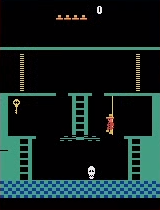
\includegraphics[width=1cm]{./imgs/mz3.png}};
		\node (frames) [fit=(frame0) (frame2), pin=above:{input sequence}] {};
		% Function
		\draw [->, thin, draw=lightgray] (frame0.east) ++(0.7,0) -- ++(2,0)
			coordinate (fn0-right);
		\draw [->, thin, draw=gray] (frame1.east) ++(0.7,0) -- ++(2,0)
			coordinate (fn1-right);
		\path (frame2.east) ++(0.7,0) edge [arrow]
			node [midway, auto=right, outer sep=0.7ex,
					pin={[pin edge=pin line]below:{unknown\\valuation function}}] {
				$f: \obsS \to \B^{\abs{\fluents}}$}
			coordinate [at end] (fn2-right) ++(2,0);
		% Output
		\begin{scope}[every matrix/.style={
			matrix of nodes, nodes in empty cells,
			row sep=-\pgflinewidth, column sep=-\pgflinewidth,
			nodes={anchor=center, draw, minimum width=1.1em, minimum height=1.1em,
				font=\footnotesize, inner sep=3pt, fill=white},
			cells={draw},
		}]
			\matrix (values0) [right=of fn0-right, nodes={draw=lightgray, thin}] {
				\\\\\\\\\\
			};
			\matrix (values1) [right=of fn1-right, nodes={draw=gray, thin}] {
				\\\\\\\\\\
			};
			\matrix (values2) [right=of fn2-right] {
				1\\1\\0\\1\\0\\
			};
		\end{scope}
		\node (values) [fit=(values0) (values2), pin={output trace}] {};
		% Constraint
		\draw (values2.east) ++(0.5,0) edge [thick, dashed]
			node [midway, auto=right, outer sep=0.7ex,
					pin=below:{temporal constraint}]
				{$\trace \models \constraintS$}
			coordinate [at end] (line-right) ++(2,0);
		\node (formula) [right=0.5cm of line-right] [pin=above:{\ldl{} formula}]
			{\constraintS};
	\end{tikzpicture}
	\caption{} % TODO
	\label{fig:generic-weak-constraints}
\end{figure}
At each timestep, the same valuation function is applied to the current
observation, which is a frame of the game, in order to compute a
configuration of the fluents. This sequence of assignments, a trace, needs to
be consistent with the temporal constraint~$\constraintS$. As noted in the
previous section, there will be a huge number of possible functions, and lots
of them will respect the specification, by chance.

For each fluent $\fluent \in \fluents$, we're trying to learn a function
$f_{\fluent}: \obsS \to \B$ that is able to compute a truth value from each
input image. For simplicity, we'll only focus on environments that provides a
static view of the game. This will greatly simplify the training of our model,
because a dynamic view

A temporal constraints aren't definitions; they are just minimal constraints.
We need additional clues: visual description of fluents.
Now follow my assumptions:

% TODO: \item Local propertes (with regions I don't have to find elements in a
	% frame).
% TODO: \item The property is visually apparent, inside the region.


% TODO: link to chapter where relax the assumptions and other ideas for
% stronger grounding

\section{General structure of the model}

Illustration and general description of the model.

\section{Encoding}

Encoder: the model, how it works, what does it learn, size of the encoding.

References:
Training Restricted Boltzmann Machines and Deep Belief Neworks
\cite{bib:rbm-training}\cite{bib:ml-book-murphy}.

\subsection{Model: Deep Belief Network}

\subsection{What does it learn}


\section{Boolean functions}

The fluents are true in a set of those configurations.

\subsection{Learning with genetic algorithms}

Ideas from concept learning; genetic algorithm.

References:
Genetic Algorithms for Concept learning\cite{bib:ga-for-concepts},
Genetic Algorithms review\cite{bib:ga-mutations-review}.

\subsection{Boolean rules}

Representation of boolean functions and training details.

\section{Limitations and improvements}

\label{sec:fluents-limitations}

% TODO: improve: maybe also some labels?
% TODO: over temporal constraints alone

% TODO: unsure about representable with conjunction, because DBN is
% unsupervised
